\documentclass[conference]{IEEEtran}
\IEEEoverridecommandlockouts
% The preceding line is only needed to identify funding in the first footnote. If that is unneeded, please comment it out.
%Template version as of 6/27/2024

\usepackage[spanish]{babel}
\renewcommand\spanishtablename{Cuadro}

\usepackage{cite}
\usepackage{url}
\usepackage{amsmath,amssymb,amsfonts}
\usepackage{algorithmic}
\usepackage{graphicx}
\usepackage{textcomp}
\usepackage{xcolor}
\def\BibTeX{{\rm B\kern-.05em{\sc i\kern-.025em b}\kern-.08em
    T\kern-.1667em\lower.7ex\hbox{E}\kern-.125emX}}


%\usepackage{fancyhdr}
%\fancyhead[L]{ }
%\lhead{\hspace{-1.5cm}\includegraphics[width=.7\textwidth]%{lheader2021}~}
%\rhead{\includegraphics[width=.3\textwidth]{rheader2021}}
%\rfoot{Página \thepage ~de \pageref{LastPage} }
%\fancyfootoffset{1.5cm}
%\lfoot{\includegraphics[width=1.2\textwidth]{footer2024}}
%\cfoot{}

\graphicspath{{./images/}}

\begin{document}

\title{\LARGE Universidad Autónoma Metropolitana Unidad Iztapalapa\\
{\Large Licenciatura en Ingeniería Biomédica\\
Reporte de prácticas de laboratorio\\
Secuenciadores y Microprocesadores 24-P}
}

\author{\IEEEauthorblockN{1\textsuperscript{st} Omar Piña-Ramírez}
\IEEEauthorblockA{opina.ramirez@izt.uam.mx}
\and
\IEEEauthorblockN{2\textsuperscript{st} Omar Piña-Ramírez}
\IEEEauthorblockA{delozath@xanum.uam.mx}
\and
\IEEEauthorblockN{3\textsuperscript{rd} Given Name Surname}
\IEEEauthorblockA{\textit{dept. name of organization (of Aff.)} \\
\textit{name of organization (of Aff.)}\\
City, Country \\
email address or ORCID}
}

\maketitle

\begin{abstract}
Plantilla de \LaTeX para realizar reportes de prácticas pensado para la división de Ciencias Básicas e Ingeniería de la Universidad Autónoma Metropolitana Unidad Iztapalapa. Este documento está basado en la plantilla \textit{IEEEtran} la cual se puede descargar íntegramente desde \url{https://www.ieee.org/conferences/publishing/templates.html}. Esta plantilla para reportes aún se encuentra en desarrollo v0.5, rev2.0.
\end{abstract}

\begin{IEEEkeywords}
Palabras clave.
\end{IEEEkeywords}

\section{Introducción}
Lorem ipsum dolor sit amet, consectetur adipiscing elit. Ut tempor mauris lacinia massa scelerisque blandit. Vestibulum ultricies ligula at libero molestie, sit amet suscipit velit elementum. Maecenas consectetur dictum dignissim. Praesent consectetur tristique ultricies. Ut elementum purus eget lacinia tempus. Nulla vitae nunc pharetra, semper enim nec, malesuada sem. Suspendisse quis leo libero. Nunc sapien justo, luctus ornare congue a, interdum ut tellus. Vestibulum feugiat tempus fermentum. Pellentesque convallis nisl ante, sit amet elementum nulla congue ac.

\subsection{Subsecciones}
Cras pulvinar non urna non ornare. Sed condimentum ante sit amet ante efficitur luctus. Proin ut purus vel dolor lacinia egestas. Vestibulum venenatis sem felis. Phasellus ac interdum magna. Praesent ac nisi tellus. Vestibulum iaculis orci in consectetur dignissim. Etiam erat urna, feugiat at sem ut, laoreet lacinia diam. Donec cursus sed tellus eu ornare. Quisque feugiat quam lectus. Ut consectetur nisi non fermentum iaculis. Pellentesque vel sodales sapien, non lacinia massa. Nunc mattis, neque sit amet maximus suscipit, nibh risus congue tellus, at finibus velit quam non dolor. Nullam vehicula elementum turpis, in molestie est bibendum vitae.

\section{Ecuaciones}
Ejemplo de ecuación y su referencia~\eqref{eq:1}
\begin{equation}
y(x) = \sum_{i=1}^N -\dfrac{1}{\gamma} x_i^2 \label{eq:1}
\end{equation}


\section{Figuras y Cuadros}\label{FAT}
Fig.~\ref{fig:1} es un ambiente para figuras que pueden ir a una columna; mientras que Fig.~\ref{fig:2} muestra el ambiente para mostrar una figura a dos columnas. Los formatos de imágenes aceptados son PNG y JPG. Al invocar \textit{includegraphics} se utiliza el nombre del archivo sin la extensión.

\begin{figure}[htbp]
\centering

\includegraphics[width=0.45\textwidth]{fig1}
\caption{Figura a una columna. Logotipo de UAM-Iztapalapa extraído del manual de identidad gráfica 2016.}
\label{fig:1}
\end{figure}

\begin{figure*}[htbp]
\centering
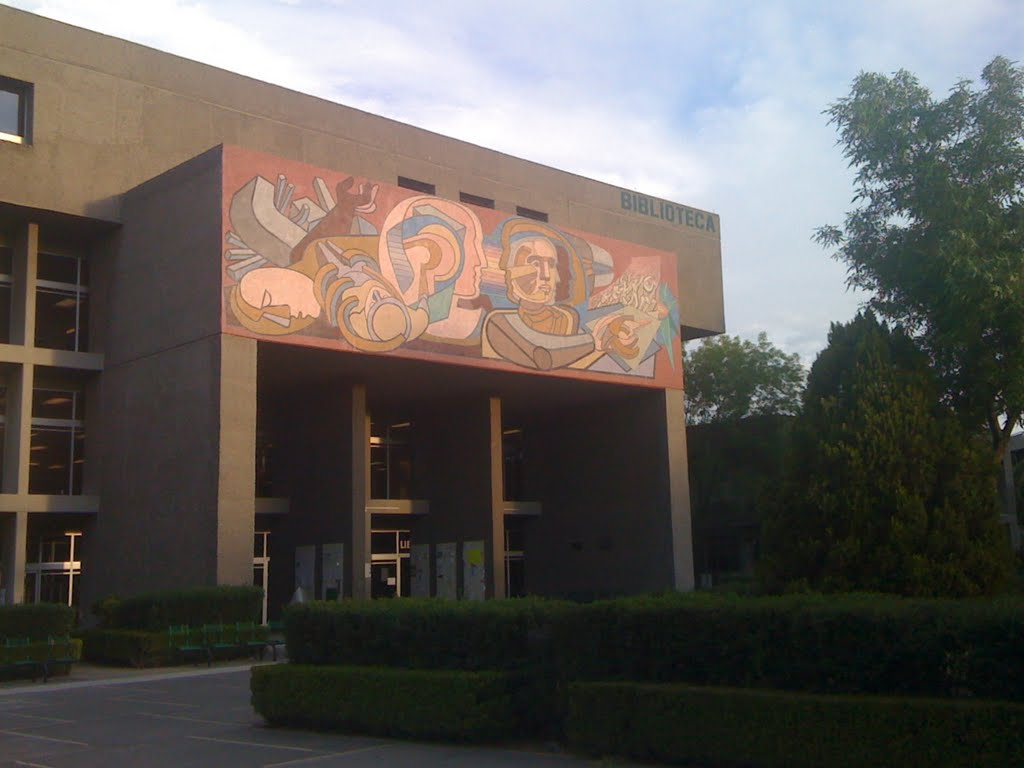
\includegraphics[width=0.7\textwidth]{fig2}
\caption{Figura a dos columnas. Biblioteca de UAM-Iztapalapa}
\label{fig:2}
\end{figure*}

\LaTeX se encarga de ordenar los Cuadros y las Figuras, por lo tanto únicamente se requiere ubicar en el código el lugar en donde aparecerán dichos elementos.

Los cuadros también se pueden disponer a una (Cuadro~\ref{tab:1}) a dos columnas (Cuadro~\ref{tab:2}). En línea existen generadores de cuadros con sintaxis \LaTeX por ejemplo \url{https://www.tablesgenerator.com/}.

\begin{table}[htbp]
\caption{Cuadro a una columna.}
\begin{center}
\begin{tabular}{|c|c|c|c|}
\hline
\textbf{Table}&\multicolumn{3}{|c|}{\textbf{Table Column Head}} \\
\cline{2-4} 
\textbf{Head} & \textbf{\textit{Table column subhead}}& \textbf{\textit{Subhead}}& \textbf{\textit{Subhead}} \\
\hline
copy& More table copy$^{\mathrm{a}}$& &  \\
\hline
\end{tabular}
\label{tab:1}
\end{center}
\end{table}

\begin{table*}[htbp]
\caption{Cuadro a dos columnas.}
\begin{center}
\begin{tabular}{|c|c|c|c|}
\hline
\textbf{Table}&\multicolumn{3}{|c|}{\textbf{Table Column Head}} \\
\cline{2-4} 
\textbf{Head} & \textbf{\textit{Table column subhead}}& \textbf{\textit{Subhead}}& \textbf{\textit{Subhead}} \\
\hline
copy& More table copy$^{\mathrm{a}}$& &  \\
\hline
\multicolumn{4}{l}{$^{\mathrm{a}}$Nota al pie de un cuadro.}
\end{tabular}
\label{tab:2}
\end{center}
\end{table*}

\section{Referencias}
El formato de las referencias es bibtex para esta plantilla basada en la de IEEE template no es compatible con biblatex~\cite{Donald1986,Mittelbach2004}. Únicamente se necesita agregar al archivo \textit{references.bib} el cual se puede gestionar desde jabref \url{https://www.jabref.org/}.

Otros dos ejemplos de referencias para un libro~\cite{Stallings2009} y para un \textit{proceedings}~\cite{Pina-Ramirez2006}.


%\bibliographystyle{unsrt}
\bibliographystyle{ieeetr}
\bibliography{references.bib}

\end{document}
